\section{Introduction}
The work presented in this thesis, being experimental in nature, hinges on numerous experimental techniques. The fundamental components of this work rely upon extensive use of X-ray diffraction (XRD) and transmission electron microscopy (TEM) in non-standard and novel ways. These techniques will be examined and examined in some detail, as their novel usage is integral to the work presented here. Several other experimental techniques are also utilized in this work, but they are used in their everyday implementations as seen in many papers in literature. These experimental techniques will be discussed only briefly for brevity. The two primary growth techniques used in this work will also be described, however as this work concentrates on epitaxy is a general phenomenon the intricacies and parameter spaces of these techniques will not be considered again for brevity.

\section{X-Ray}
X-rays are high energy photons, generated from the transitions of electrons between their core shell energy levels and bremsstrahlung (the acceleration of electrons). X-rays have a relatively weak interaction with matter, being absorbed or perturbed only slightly upon passing through it. X-rays have wavelengths comparable with the typical spacings between atoms in crystals, placing them as an ideal non-destructive probe for crystal structure. X-rays experience elastic scattering when interacting with the electrons surrounding atoms. The scattering of x-rays, combined with the 3D periodic structure of atoms, results in constructive and destructive interference and x-ray diffraction.
\begin{equation}
\label{eqn:bragg} 2d \sin(\theta) = n \lambda
\end{equation}
X-ray diffraction is fundamentally an interference phenomenon, for a set of planes within a crystal separated by some distance (d), they will diffract from those planes at an angle (\texttheta) depending upon the wavelength (\textlambda), this is known as Bragg's law as in \cref{eqn:bragg}. Bragg's law is identical to the phenomenon of thin film interference of visible light, only differing by the scale of the spacing and wavelengths. Bragg's law, while correct, is a one dimensional expression, in general it can be represented by the Laue Equations as in \cref{eqn:laue}. The vectors $k_i$ and $k_0$ are the incident and outgoing x-ray beam, $(a,b,c)$ is the primitive vector of the crystal lattice and $(h,k,l)$ are the reciprocal lattice indicies which must be integers. Thus, for a given crystal with a fixed unit cell, there are only certain relationships between the incident and outgoing x-ray beams that satisfy the diffraction conditions, resulting in diffraction.
\begin{align}
   a \cdot (k_0 - k_i) = 2 \pi h \\
   b \cdot (k_0 - k_i) = 2 \pi k \\
   c \cdot (k_0 - k_i) = 2 \pi l
   \label{eqn:laue}
\end{align}

A concept known as reciprocal, or momentum space, is a common construct used in solid state physics to discuss the properties of crystals and is intimately related to diffraction. Reciprocal space can be visualized as a lattice of points, each representing a spacing present in the crystal, and the lattice having the same symmetry as the real crystal. Reciprocal space is also the Fourier partner of the real space lattice of the crystal. Reciprocal space provides an opportunity for an alternate expression of the conditions for diffraction, known as the Ewald construction. The Ewald construction or Ewald sphere expresses the diffraction condition through the overlay of a sphere of radius 1/\textlambda{} pinned on its radius at the origin in reciprocal space, a incident X-ray beam ($k_i$) entering the sphere. The direction of the exiting diffraction beam is determined by the intersection of the surface of the sphere with the reciprocal lattice, as shown in \cref{fig:exp_xray_ewald}. As a crystal is rotated (or the incoming beam is moved), the Ewald sphere will rotate about the origin, sweeping through reciprocal space and exciting diffraction conditions as the sphere coincides with lattice points. The pinned rotation of the Ewald sphere about the origin means that only reciprocal lattice points with a radius from the origin of less than 2/\textlambda{} can be excited into diffraction, indicating the effective limitation of a given x-ray source, as well as why light is an ineffective diffraction probe.
\begin{figure}
\centering
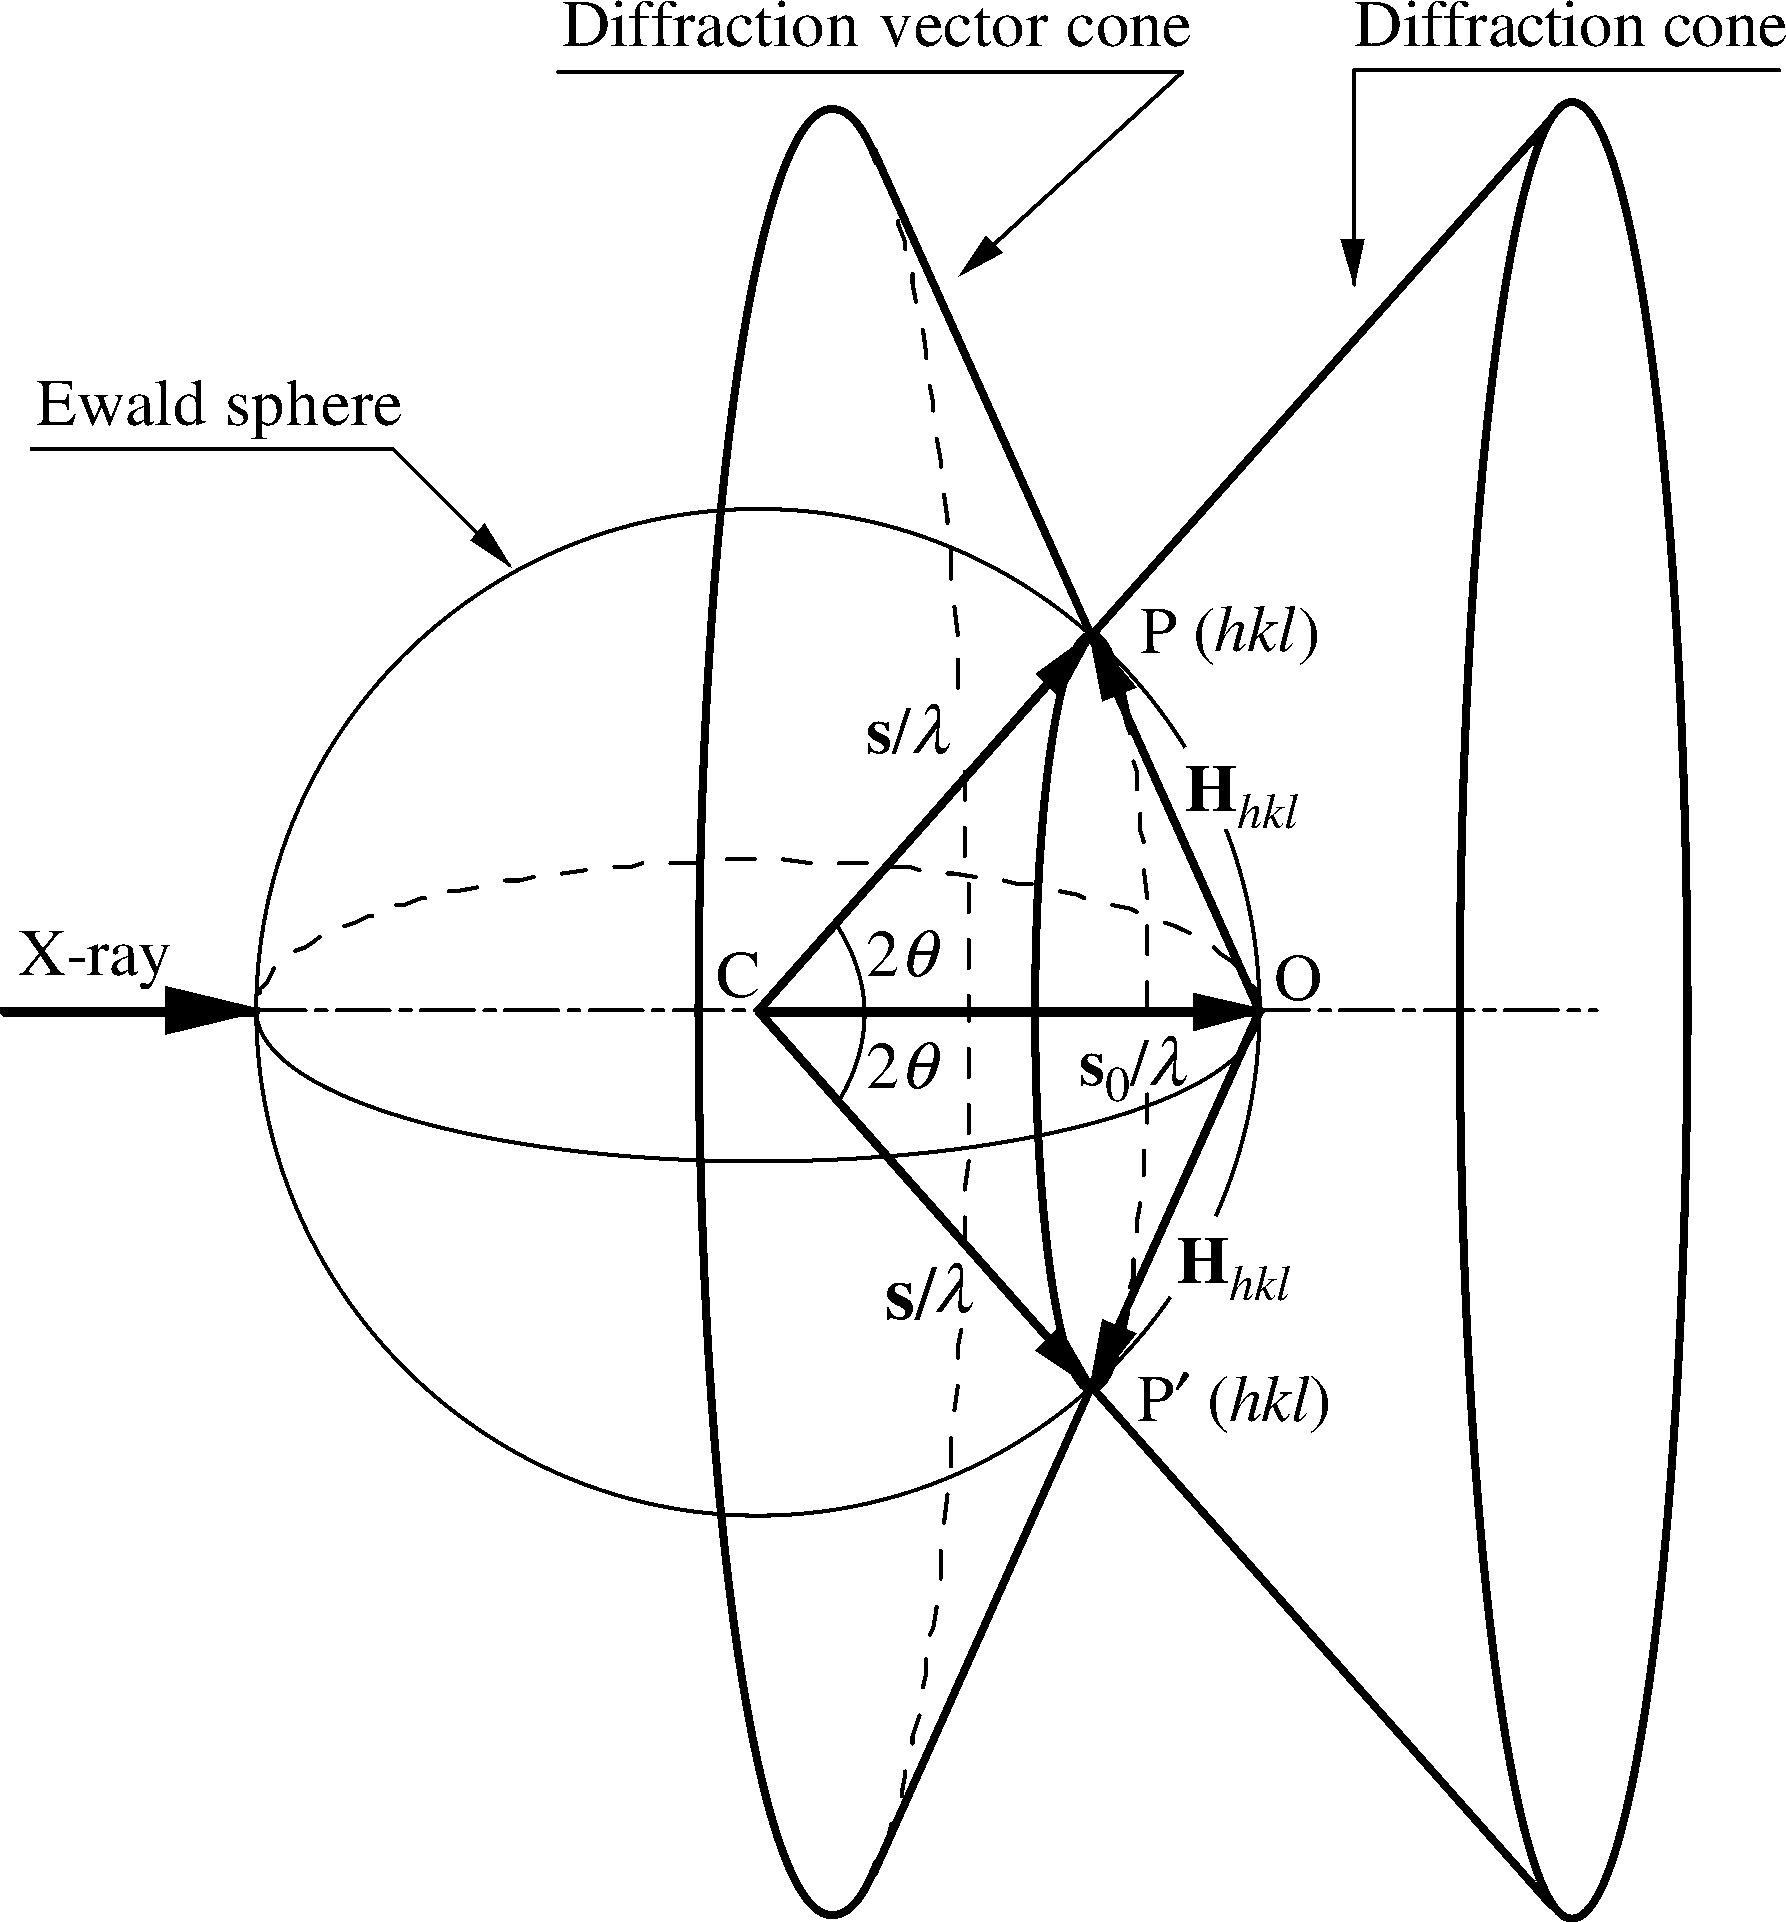
\includegraphics[width=0.6\textwidth]{exp_xray_ewald}
\caption{\label{fig:exp_xray_ewald}Ewald sphere construction of diffraction conditions\cite{bobhe}}
\end{figure}

\subsection{2DXRD - Reciprocal Space Mapping}
\label{sec:2DXRD} As shown by \cref{eqn:laue} and \cref{fig:exp_xray_ewald}, there are an large number of orientations of a crystal which generate diffraction. For the purposes of the analysis of crystals, the lowest orders of crystal diffraction (small h,k,l) are the strongest, and provide the least ambiguous information, the they are also at the lowest 2\texttheta{} values. This still leaves a significant number of diffraction beams of interest to measure and provide structural information. The naive measurement technique for collecting this information involves taking a crystal and orienting an incoming x-ray beam, and a detector in configurations that satisfy \cref{eqn:laue}. Such measurements assume that the experimenter knows the orientation and unit cell of the crystal to a degree well enough calculate those configurations. If either of those pieces of information is unknown, the experimenter must instead sample the 4\textpi{} solid angle (usually only the upper 2\textpi{} half) of angular space surrounding a crystal with sufficient resolution to intersect with the diffraction conditions of interest. Such experiments, when performed using a typical x-ray point detector, take inordinate amounts of time, as the angular space is large and the point detector must count for a long time to achieve good counting statistics.

An alternate implementation of such a measurement process is through the use of a 2D planar detector rather than a point detector. A 2D x-ray detector can subtend a large section the angular space surrounding a given experiment, potentially collecting information about a large section of reciprocal space with each frame it collects. If configuration is then swept through a range of diffraction conditions, the 2D detector will collect information about a wide swath of reciprocal space. 2DXRD techniques simultaneously collect information about the phase and symmetry of an unknown sample allowing that information to be then examined via a variety of techniques.

\subsubsection{Practical 2DXRD Measurement}
\begin{figure}
    \centering
    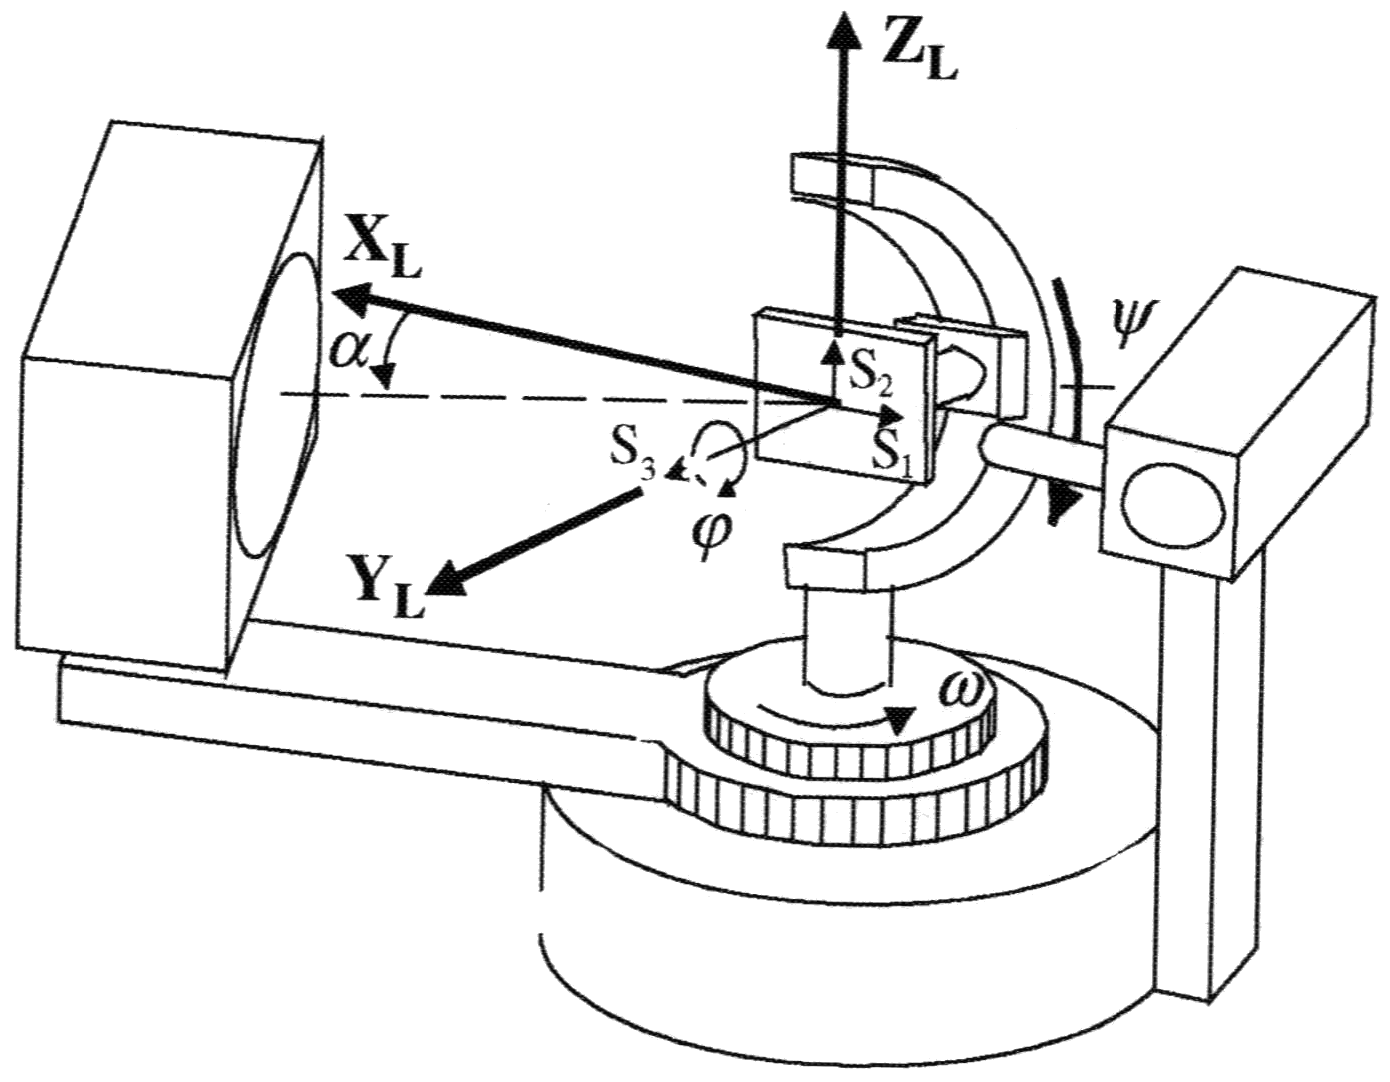
\includegraphics[width=0.8\textwidth]{exp_xray_machine}
    \caption{\label{fig:exp_xray_machine}Standard configuration of a 2DXRD system, with the laboratory geometry\cite{bobhe}}
\end{figure}
Practical 2DXRD measurements are achieved through the use of a multi-axis goiniometer, a device which maintains the sample at a central point while rotating its orientation relative to the X-ray source and detector. For the purposes of epitaxial crystals grown on substrates, a sample under measurement is placed in the goinometer with its surface normal oriented along the goiniometer's sample axis and a reference edge. An x-ray source is placed on one arm of the goiniometer and the 2D detector is placed on the other arm.

A standard 2DXRD measurement is performed by configuring the goiniometer (\cref{fig:exp_xray_machine}) such that the X-ray source to 2D detector angle corresponds to a known or presumed low-order 2\texttheta{} angle for the sample. The sample was then rotated such that incident angle relative to the surface is shallow, less than 5\degree{}. The sample would then be rotated about its surface normal while the 2D detector took sequential images, a process known as a \textphi{}-scan. By aligning the sample along 2\texttheta{} in one dimension, as the sample rotates in a complimentary dimension crystallographic directions that contain the d-spacing corresponding to a range of 2\texttheta{} around the selected value will be collected on the detector. The number of frames exposed during this rotation determines the resolution along the rotation direction in reciprocal space, while the resolution of the 2DXRD detector determines the complimentary dimension. An additional scan of the sample while maintaining the 2\texttheta{} configuration and scanning the X-ray beam incident angle is known as an \textomega{}-scan. While the combination of these two scans collects only the reflections surrounding the centred 2\texttheta{} of interest, if the measurement scheme successfully collects all or the vast majority of the reflections, the symmetry of the underlying system will allow any other reflections to be inferred, greatly reducing overall measurement time.

As the reciprocal space mapping is a process which operates in angular space, the distance the detector is an important optimization parameter for 2DXRD measurements. The distance the 2DXRD detector is situated away from sample will change the solid angle subtended by the detector. Close detector distances allow the collection of more reciprocal space data in a given scan, at the expense of reducing the resolution due to finite pixel size, as well as increasing the risk of overlap. For epitaxial thing films grown on lattice mismatched substrates, close detector distances can result in substrate and epitaxial crystal peaks overlapping, making interpretation difficult.

The last optimization parameter for 2DXRD scans is the amount of time spent collecting each frame. For a given brightness of x-ray source and thickness of material, the frame exposure times are ideally set to capture counts just below the maximum the electronics can achieve. Maximizing the counts for the x-ray detector ensures optimum signal to noise for a given measurement.

\todo{Show/calculate area exposed by x-ray beam}

\subsubsection{Interpretation of 2DXRD Measurements}
Once a 2DXRD measurement has been taken, the resulting data consists of a series of 2D detector frames. The exact number of frames is determined by the sampling resolution set during the 2DXRD scans. Each frame is a snapshot of the the diffraction intensity collected from the sample for the exact angular configuration in space stored with the frame. A single 2DXRD frame (\cref{fig:exp_xray_frame}) which contains a x-ray diffraction peak can be analyzed via a number of integration techniques. The two perpendicular pixel directions on the 2DXRD frames are transformed into two angular dimensions in the coordinate system of the sample, 2\texttheta{} and \textchi \cite{bobhe}. The resulting frame is sliced into hyperbola with the x-direction of the frame corresponding to the radius and a new dimension \textchi{} corresponding to the direction along a given hyperbola.
\begin{figure}
    \centering
    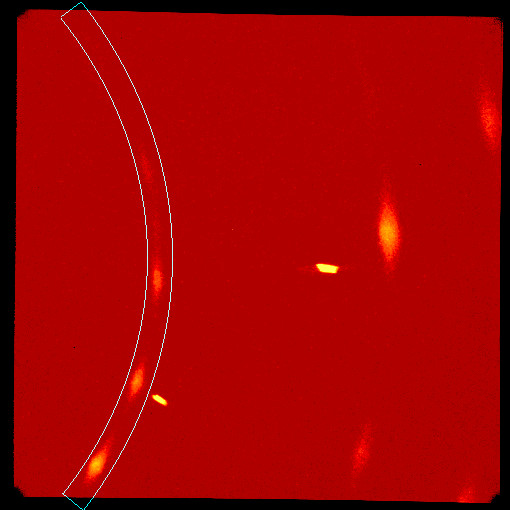
\includegraphics{exp_xray_frame}
    \caption{\label{fig:exp_xray_frame}An example x-ray frame with a conic section of fixed 2\texttheta{} highlighted}
\end{figure}

The data on a frame can be integrated in one dimensional plots along either dimension of the hyperbola. Integration of the data along \textchi{} and plotting with respect to 2\texttheta{} results in a pseudo-powder pattern similar to those taken in a common Bragg-Brantano XRD system, expect it can be performed for diffraction peaks other than perpendicular to the substrate. Such plots show the presence of d-spacings within the frame of interest, and their width. Integration of data over a 2\texttheta{} range and producing a one dimensional plot will show the spatial intensity distribution of a given diffraction peak. Examples of both such integration types are shown in \cref{fig:exp_xray_frame}.

\subsubsection{Pole Figure Generation}
While integration of the diffraction data on a single frame provides useful quantitative measures of the distribution of a diffraction peak in space, when many frames are collected the generation and interpretation of many frames is tedious difficult to interpret. Pole figure generation from a set of frames is a method of graphically representing the spatial extent of the diffraction intensity of a given d-spacing around a given sample. Pole figures readily allow the interpretation of diffraction data to assess crystalinity, presence of phases and orientation relationships between a substrate an epitaxial crystal.
\begin{figure}
    \centering
    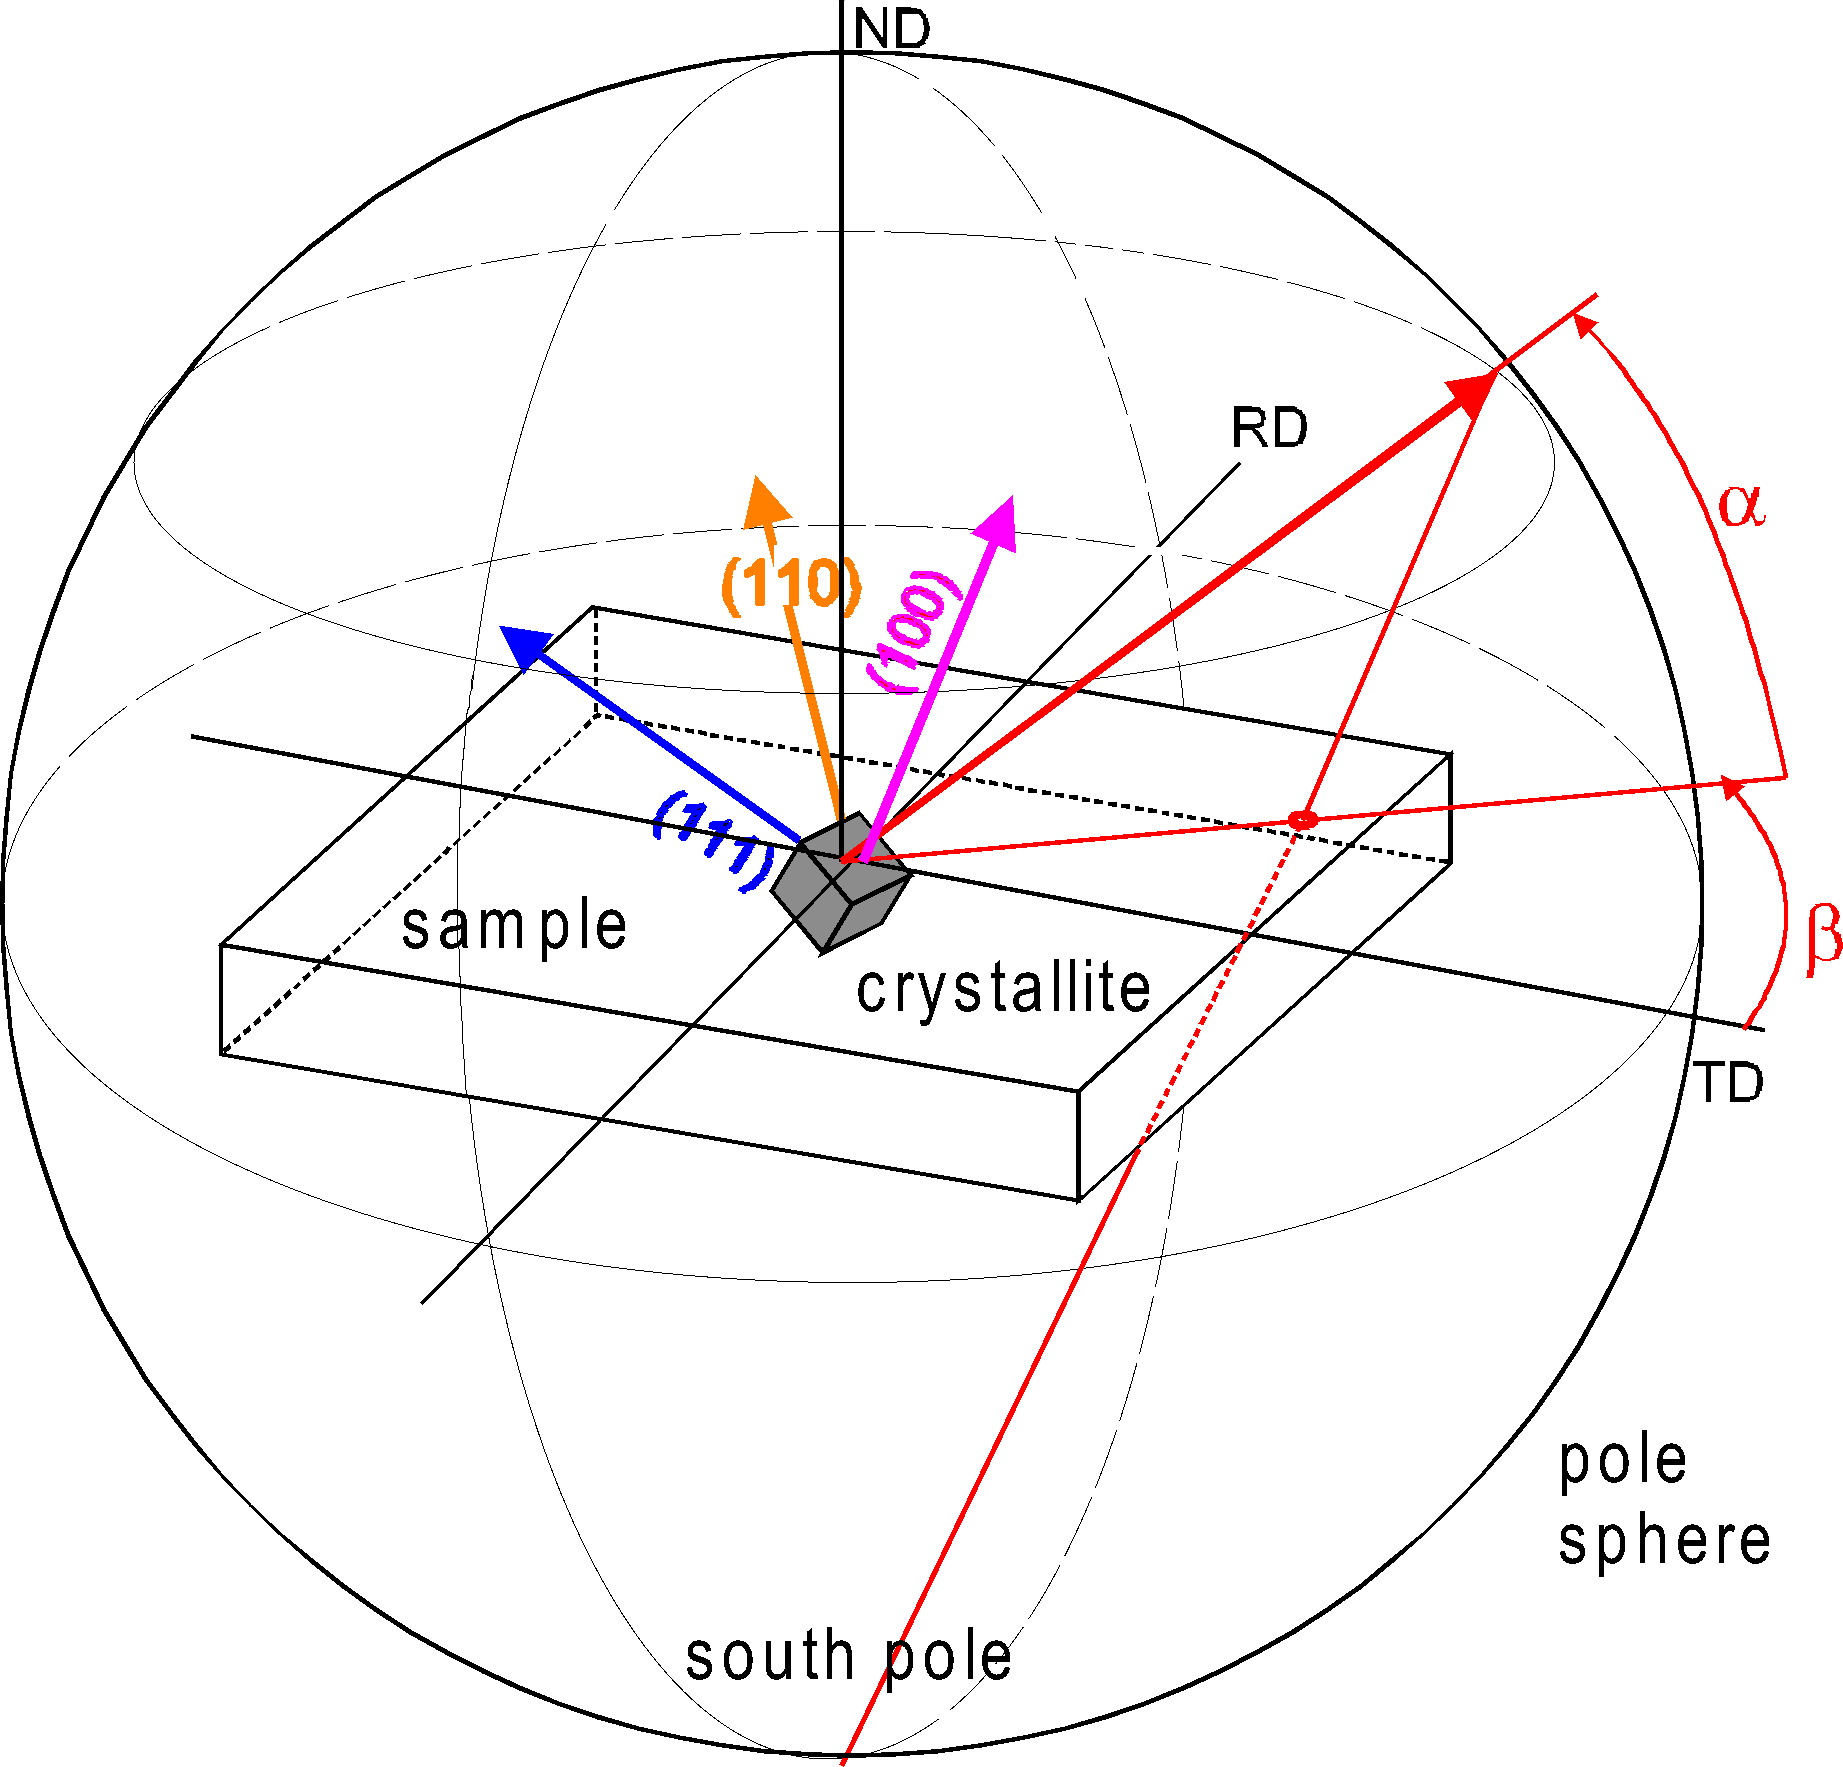
\includegraphics[width=0.7\textwidth]{exp_xray_polesphere}
    \caption{\label{fig:exp_xray_polesphere}The pole sphere showing the origin of peaks in a pole figure and their relationship to the sample and an individual unit cell\cite{gadds_manual}}
\end{figure}

To generate a pole figure from a collection of frames a 2\texttheta{} and \textchi{} range are selected on the first frame of a series of frames. Generally, such a range will include the maximum width of a single d-spacing of interest (such as \{111\}) and the entire extent of \textchi{} on the frame. The range is integrated across 2\texttheta{}, producing a one dimensional intensity scan. The intensity scan from each frame is then mapped onto the pole sphere (\cref{fig:exp_xray_polesphere}) according to the frame orientation information, forming a geodesic line of intensity. The pole sphere is a construction centred on the sample which maps the direction in space that diffraction intensity is collected by the detector. As each frame is integrated, the surface of the pole sphere is painted with colour mapped intensity data. The resulting sphere of data is then stereographically (angle preserving) projected onto a circle, resulting in a pole figure. The pole figure is a polar diffraction intensity colour map with the radial direction represented by \textalpha{}, the angle from the top of the sphere and the azimutual direction \textphi{} is the in-plane orientation relative to the sample's \textphi{} zero orientation set during sample mounting. An example pole figure mapping a single data point from the pole sphere is shown in \cref{fig:exp_xray_polefigure}. 
\begin{figure}
    \centering
    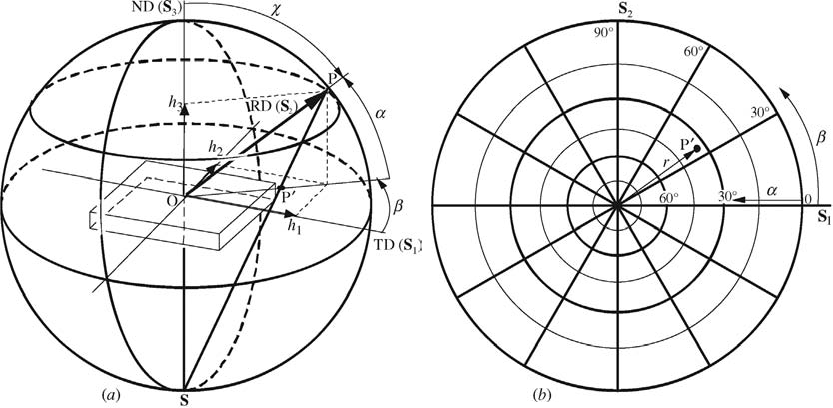
\includegraphics[width=\textwidth]{exp_xray_polefigure}
    \caption{\label{fig:exp_xray_polefigure}Example mapping of pole sphere data points to pole figure\cite{bobhe}}
\end{figure}

\subsubsection{Ipretation and Simulation of Pole Figures}
Once a pole figure has been generated the resulting graphical representation of the diffraction data must be interpreted in the context of the sample. Generally, a pole figure will be generated for a low-index reflection (100,110,111) for both the epitaxial crystal and the substrate. By generating two figures, the orientation relationship between the diffraction intensity produced by the grown crystal and the single crystal substrate can be examined by comparing the two figures.
\begin{figure}
    \centering
    \missingfigure{Comparison of Winwulff simulation and generated single crystal silicon (111) pole figure}
    \caption{\label{fig:exp_xray_winwulff}Comparison of Winwulff simulation and generated single crystal silicon (111) pole figure}
\end{figure}

The first step for pole figure analysis is to examine the pole figure generated from the substrate low index reflection. Since the substrate should be a single crystal, it is trivial to interpret it for its orientation information. A single crystal pole figure of the substrate can be simulated by considering the space group (cubic, hexagonal, etc.), unit cell, and physical orientation (100-up, 111-up), calculating the surface normals of the d-spacing of interest, collecting them on a pole sphere and mapping them onto a pole figure. This is conceptually identical to the generation of a pole figure from raw data, except the data is computed from a perfect crystal unit cell. Such pole figures are simulated using a piece of software such as WinWulff\cite{winwulff} as seen in \cref{fig:exp_xray_winwulff}, allowing interaction with the pole figure.  The pole figure generated from the data is then compared to the simulated pole figure and the simulation is manipulated by changing the orientation of the crystal until the two figures coincide. The orientation information provided by the simulation software is now the same as the orientation of the measured crystal. Such comparison provides the absolute orientation of the crystal in the diffractometer, and all other pole figures generated form the dataset can be referenced to that crystal.

Now that the substrate orientation is known, the pole figure generated from the data can be referenced to the substrate. If the epitaxial crystal is also a single crystal, the same trivial comparison process can be performed. The resulting orientation of the eptitaxial crystal can be compared to the substrate, providing the epitaxial relationship.

For the case of systems which have non-ideal epitaxial growth, the pole figures likely contain diffraction intensity information from a number of crystalline sources. This pole figure as the convolution of the pole figures for each of the components of the epitaxial crystal. There are several features which arise in such pole figures which are characteristic of certain growth relationships. A pole figure that, when generated, is uniform in intensity, or has intensity present everywhere with a broad distribution is characteristic of a strongly polycrystalline growth random in orientation, with no epitaxial relationship to the substrate, a simulated pole figure of such a situation is shown in \cref{fig:exp_xray_polefigure_examples}a. Pole figures which contain bands of diffraction intensity which are rotationally symmetric about their centre are characteristic of a crystal that has a preferred stacking order in the vertical direction, but has no in-plane orientation, such an example is shown in \cref{fig:exp_xray_polefigure_examples}b. Such preferred stacking orders, usually (111)-up is a common occurrence when growing binary cubic materials.

The most difficult situation that occurs is when the generated pole figure contains multiple single crystal-like peaks. The presence of single crystal-like peaks indicates a number of different orientations of the crystal of the epitaxial crystal. These epitaxial crystals are referred to as textured materials, an example of which is shown in \cref{fig:exp_xray_polefigure_examples}c. For textured epitaxial crystals, there are number of possibilities for the cause of texturing during growth. Many FCC binary semiconductors have a propensity to have stacking faults or twins during growth. The twinned crystallite will create new diffraction peaks in the pole figure, they will have a twin relationship with the host crystal about the twin direction (usually \{111\}).

Other textured epitaxial crystals may arise through multiple preferred growth relationships with the underlying substrate. Such systems typically have pole figures where the symmetry of the overall pole figure reflects the substrate surface symmetry. The example in \cref{fig:exp_xray_polefigure_examples}c is one of a (111)-up crystal (3-fold symmetry) on a (100) substrate (4-fold symmetry), showing $3\times 4=12$ peaks.
\begin{figure}
    \centering
    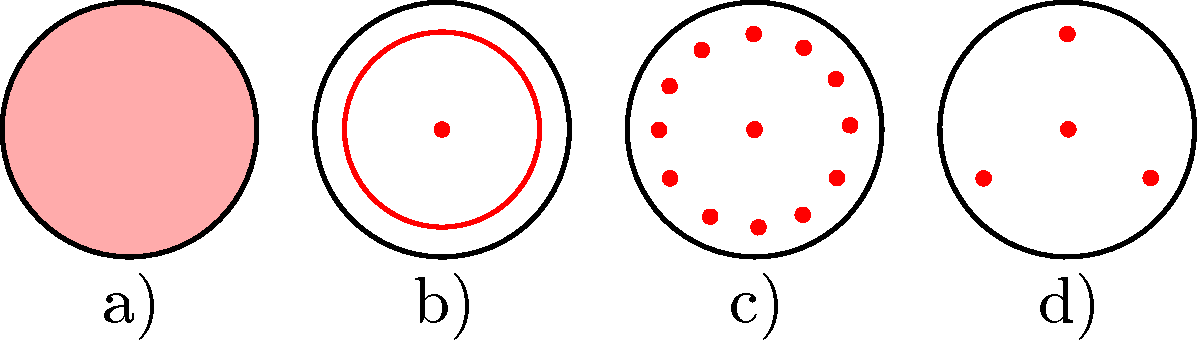
\includegraphics{exp_xray_polefigure_examples}
    \caption{\label{fig:exp_xray_polefigure_examples}Example pole figures of a) Polycrystalline randomly oriented b) in-plane random orientation c) textured epitaxial crystals of the same composition and crystal structure}
\end{figure}

Beyond the analysis of the symmetry of diffraction intensity, which indentifies the crystallites present within a sample, the relative intensities within the pole figure provide a wealth of information about the epitaxial crystal. Similar to the integration techniques applicable to raw 2DXRD frames, the diffraction intensity in a pole figure can be sliced and integrated in a number of ways. The pole figure can be inspected by simply integrating the information in a given area, allowing comparison of the intensity of individual diffraction peaks. Pole figure intensity can also be integrated radially and plotted versus \textphi{}, providing information on the in-plane rotational misalignment of the selected epitaxial crystallites. Finally, pole figure intensity can be integrated versus \textphi{} and plotted radially.

Plots of radial data from pole figures are particularly informative, broadening of diffraction peaks preferentially in the radial dimensions is a indication of strain present in a crystallite. The radial location of a peak in a pole figure is determined by the unit cell and the orientation of the crystal. Radial broadening in a pole figure is an indication that the unit cell has been distorted relative to it's preferred shape.

\subsection{High Resolution XRD}
While mapping reciprocal space provides a great deal of information about the phases and symmetries present in a given sample, the resolution available on such 2D detectors is limited in both the number of pixels, and the spacing between them. In addition, the x-ray beam geometry associated with 2DXRD measurements introduces instrumental broadening into the measurements preventing careful inspection of small scale diffraction details. In order to examine the small scale details of diffraction intensity, a different configuration must be implemented for the x-ray source and detector, this configuration is known as high resolution x-ray diffraction. If the general landscape of reciprocal space (diffraction intensity) is known through the application of 2DXRD techniques, HRXRD can carefully sample small sections of reciprocal space with very high resolution.

Recall that for a perfect crystal, there is only a single configuration for which the diffraction condition will be satisfied, resulting in a highly intense diffraction peak with minimal spacial extent. For a real sample, intensity distribution of individual diffraction peaks in reciprocal space provides information about the deviance from the ideal crystal.

Using HRXRD measurements, the exact d-spacing of a given material can be determined, showing whether a sample has its lowest energy structure or it is strained. If the orientation of the sample can be controlled carefully, the d-spacing can be measured absolutely, otherwise, it can be measured relative to a known standard such as a single crystal substrate. The broadening (spatial extent) of a HRXRD peak provides different information depending upon the dimension along which it is examined. In the 2\texttheta{} direction, the radial direction in reciprocal space, broadening indicates that the spacing of interest is actually a distribution of spacings within the region of the sample illuminated by x-rays. Such distributions can indicate strain or compositional variation in the region of interest. The broadness of the x-ray peak when sample is rocked in the \textomega{} direction, while keeping 2\texttheta{} fixed indicates that a given d-spacing has a distribution of orientations within the sample, usually indicating multiple crystallites.

\subsubsection{Practical HRXRD Measurement}
In order to ensure the validity of HRXRD measurements of exact d-spacings and x-ray diffraction peak widths, the HRXRD system and it's operation must satisfy several conditions. These properties specifically deal with the properties of the x-ray source used in HRXRD, and the operation of the goiniometer in the rotation of the sample, source, and detector.

For practical HRXRD, the x-ray source much monochromated far more than for general x-ray work. Typical x-ray sources will contain bright peaks from multiple core electron levels, along with Bremsstrahlung radiation, and will be monochromated with a one monochromator. Such a source will still have an appreciable broadening in its peak and such broadness will convolve with the sample's true properties. HRXRD measurements must be taken with x-ray sources with at least two monochromators, and may have up to four. Sufficient monochromation will ensure that the instrumentation broadening will be below the level of the sample's actual diffraction properties, allowing a sensible measurement result. Such extra monochromation results in a significantly weaker signal than general experiments, and a much longer experiment time. Beam size considerations are a balance between the sample's spatial distribution and the intensity of the diffraction signal.

The second practical requirement for HRXRD is for precise alignment of the sample, and the ability to be make precise movements of the sample. Absolute alignment of the sample is required in order to absolutely determine the orientation of crystal structures and the d-spacing of the planes of interest. Precise orientation and movement of sample is achieved by a goniometer with resolution of at least one arcsecond (1/3600 of a degree), with good reproducibility.

Practical HRXRD measurements, even after performing alignment, are best performed by with reference to a known diffraction peak. For HRXRD measurements attempting to determine the exact d-spacing for a epitaxial crystal, it is best achieved by aligning to a strong reference peak of the substrate, and including that peak in the measurement in order to allow both absolute measurement and relative calculation of the d-spacing.

\section{Electron Microscopy}
The second of two very useful probes for examining the properties of epitaxial thin films is electrons, specifically, electron beams generated for electron microscopy. The electron, unlike the x-ray is a particle which interacts fairly strongly with materials. Electrons can be generated and accelerated to high velocities, resulting in DeBroglie wavelengths orders of magnitude smaller than X-rays and as a a result can be confined or focused to sub-angstrom areas. The electron's use as a probe can be used as both a mechanism to produce excite other phenomena for study, or to measure the effect a given sample has on a beam of uniform electrons. For generic beam of nearly-monochromatic electrons, typical of electron microscopy, a number of interactions are possible for a sample of finite thickness, as shown in \cref{fig:exp_em_electron_interaction}. The interactions of electrons with a sample can provide both chemical and structural information with fine spatial resolution thanks to the tight control of electron beams.
\begin{figure}
    \centering
    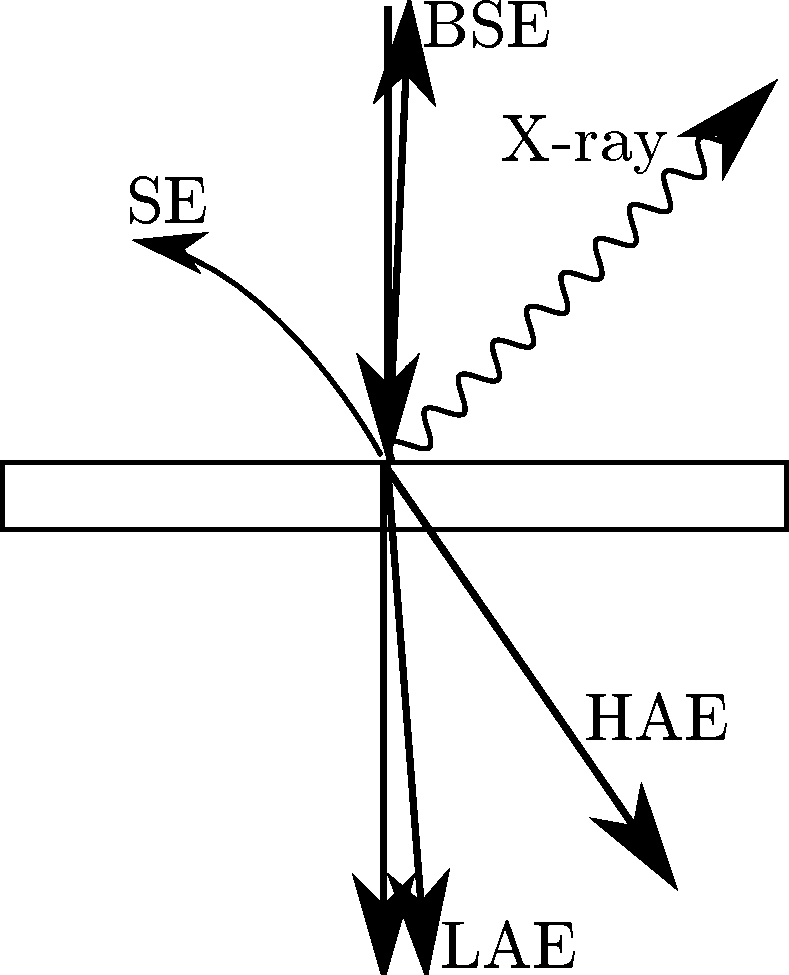
\includegraphics[width=0.7\textwidth]{exp_em_electron_interaction}
    \caption{\label{fig:exp_em_electron_interaction}Schematic of an electron beam interacting with a sample showing backscattered electrons (BSE), secondary electrons (SE), generated X-rays, low angle scattered electrons (LAE), high angle scattered electrons (HAE), and the main electron beam passing through the sample.}
\end{figure}

This work relied upon two measurement techniques which utilized electrons as their primary probe, scanning electron microscopy (SEM) and (scanning)transmission electron microscopy (STEM/TEM). SEM is an invaluable technique non-destructive technique for examining surfaces at high resolution to extract information about both the structural and chemical properties. STEM/TEM is a tool which utilizes similar interactions to examine the cross sectional structural and chemical properties of mechanically thinned slices of materials with sufficient resolution to examine individual columns of atoms in crystals.
\subsection{SEM}
Scanning electron microscopy is a high resolution non-destructive and non-contact technique used to examine the surface of a sample. SEM can provide information about the topography and chemical composition of a surface down to 10's of nanometers, and the exact chemical composition on the micrometer scale. These measurements are achieved through the interaction of a beam of nearly-monochromatic electrons generated from a heated filament or cold cathode and accelerated to kilovolt velocities in an high vacuum chamber and focused onto a sample. Magnification is achieved in SEM by careful scanning of the focused beam over a small area.

\subsubsection{Secondary Electron Imaging}
The most common electron-material interaction utilized in SEM is generation of images through the production and capture of secondary electrons. Secondary electrons are continuum (valence and conduction band electrons) excited from the sample through inelastic scattering excitations. These electrons typically have energies of 10's to low 100's of electron volts. Secondary electrons are collected by biasing a electron detector in order to electrostatically attract these low energy electrons while not appreciably affecting the incoming beam. Electron detectors are typically a phosphor screen combined with a photomultiplier tube to provide high gain. Images are formed by scanning the beam across the surface of the sample and counting the secondary electron yield for each dwell point within the scan. The resulting grid of counts is transformed into a grayscale image.

As secondary electrons are low energy, their escape depth from a surface is very shallow (< 2~nm), as such their yield is very sensitive to the local topography of the sample. Thus to the first approximation, the contrast in a grayscale image formed from secondary electrons is a representation of the topography present on the surface of the sample. Regions with vertical extent will increase the yield of secondary electrons, due to more of the sample being within nanometers of the surface. An extreme case of this is vertical edges, which will have a very high yield of secondary electrons, due to having the top and side surfaces both yielding secondary electrons.

\subsubsection{Backscattered Electron Imaging}
High energy incoming electrons can also interact with samples via elastic scattering. Electrons which are scattered at close to 90\degree{} are backscattered close to the incoming beam. By placing unbiased detector near the incoming electron beam the detector can capture backscattered electrons. The electron elastic scattering process is proportional to Z$^2$ of the sample. Thus the electron backscattering process forms an image that provides chemical contrast of the underlying sample.

\subsubsection{Practical SEM}
The practical application of SEM for imaging of samples requires the optimization of several parameters. While SEM is a non-destructive measurement technique, intentional sample preparation can vastly improve the imaging resolution and reduce noise. A key requirement for SEM samples is that the sample is suffciently conductive in order to conduct away the electrons delivered by the scanning beam. For high conductivity samples, sample preparation can be as simple as bonding to a sample holder using conductive tape or paste. Samples with poorer bulk conductivity may require conductive paste applied to contact the top surface to the sample holder. For highly insulating samples substrates are normally coated with a thin layer of high density metal (Pt, Au) or amorphous carbon in order to provide a conduction path.

Optimization of imaging for a given sample is achieved through the tuning of several imaging parameters, working distance, accelerating voltage, beam current and dwell time. For typical secondary electron imaging, the goal is to interact with the thin top surface layer with the smallest lateral beam possible. Minimization of accelerating voltage, beam current and working distance will maximize the resolution and reduce the surface interaction. Reduction of these working parameters has the side effect of reducing the signal to noise ratio (SNR) of imaging. Increasing dwell time can improve SNR, but for poorly conductive samples charge buildup will cause deflection of the incoming beam. Stacked averaging of quick scans yields improved SNR on the tradeoff of time. Interpretation of the secondary electron images in one key case is ambiguous, topographic features with vertical extent can be appear due to the human visual system to be both a depression and a bump alternately. Tilting of the sample can sometimes break the ambiguity and reveal the actual topography. Adjustment of the focus plane can also reveal the topography but only during active analysis.

Imaging of using backscattered electrons to achieve chemical composition requires optimization of the elastic scattering process from the sample. Backscattered electron yield increases with increasing accelerating voltage but also increases the area of interaction reducing resolution. The elastic scattering process is significantly less efficient than secondary electron generation, as such dwell times must be increased to yield an image. In order to obtain a true measure of chemical composition, samples for backscatter analysis should be as flat as possible, as topography can modify the yield of backscattered electrons. Such processing as polishing can improve the chemical contrast. If the measurement is intended to be non-destructive, careful correlation between backscattered and secondary electron images must be used to ignore topographic effects.
\subsection{TEM}

\subsection{STEM}


\section{Growth Techniques}
The work presented in this thesis are prepared primarily by two different growth methods, pulsed laser deposition (PLD) and molecular beam epitaxy (MBE). While these methods are quite distinct in their properties and the regimes under which they operate, the same material systems were not prepared by both systems, so direct comparisons cannot be made. Nevertheless, the differences between these growth processes will be examined in some detail to provide sufficient motivation for their choice for the given experiments.
\subsection{PLD}
\subsection{MBE}
\subsection{Thermal Dewetting}